\section{Method}

Our method, Simplicial Complex Augmentation Framework (SCAF) utilizes a scaffold structure to robustly compute a bijective map between a pair of simplicial meshes with the same connectivity. SCAF is specialized for the context of geometric optimization, i.e. we are interested in maps with low distortion and optionally satisfying a set of geometric constraints. We assume our maps are continuous and piecewise affine, i.e. the map deforms every simplex with an affine deformation. Thus, we can fully define the map using the image of its vertices.

% SCAFfolding Conforming Auxiliary Faces
 Our algorithm uses a discrete, bijective identity map (encoded as a non-overlapping and non-flipping triangle/tetrahedral mesh)  as initialization and then iteratively refines it, displacing the vertices while always ensuring that it remains bijective. Our method is composed of three stages: (1) augment the initial mesh with a scaffold, filling a bounding box around the initial map image; (2) optimize the extended mesh (scaffold included), reducing the geometric distortion of the map; (3) update the vertices and scaffold, enlarging the bounding box if necessary, to improve the quality of the triangulation. Steps (2) and (3) are iterated until the quality of the map is deemed sufficient.  

\subsection{General Formulation} \label{sec:general_form}
Denote the input simplicial mesh by $\Mesh = (\V,\F)$ with a single, simple boundary representing a compact $d$-dimensional manifold embedded in the $d$-dimensional Euclidean space, where $\V$ is the set of $n$-vertices and $\F$ is the set of $m$-simplices. Our goal is to compute a continuous and piecewise affine mapping 
$\Phi : \Mesh \rightarrow \R^{d}$ with $\Omega := \Phi(\Mesh) = (\V',\F)$ the resulting simplicial mesh with the same connectivity as $\Mesh$. 

We are interested in the bijective map that minimizes a given type of geometric energy:
\begin{align}
\begin{split}\label{eq:bijective_energy}
    \min_{\V'}& \quad E_{\Mesh} (\Phi) \\
    \text{s.t.}& \quad \Phi\text{ is bijective},
\end{split}
\end{align}
where $E_{\Mesh}$ is a user-defined geometric energy.

\paragraph{Reduction to Local Orientation Preservation.}  A sufficient %\revision{and necessary} 
condition for the simplicial map 
$\Phi: M\rightarrow \Omega $ to be bijective is that the map preserves orientation and its restriction to the boundary $\Phi|_{\partial M} : \partial M \rightarrow \partial \Omega$ is bijective~\cite{Lipman:2013ArXiv}. In this light, we are able to take advantage of the following simple construction (Figure \ref{scaf:fig:construction}): the algorithm extends the axis aligned bounding box of $M$ to get a $d$-orthotope and fills the enclosed region with a scaffold simplicial complex to form a simplicial complex mesh $D$ that includes and conforms to $M \subset D$. We can now define the continuous and piecewise affine map $\Psi : D \rightarrow D'$ with $\Phi = \Psi |_{M}$ where $\Psi|_{\partial D}$ is the identity map, and denote the scaffold region as $S = D\setminus M$. Now $\Phi$ is guaranteed to be bijective if $\Psi$ preserves orientation. Using this observation, we can translate the bijectivity into a local, orientation-preserving requirement defined per simplex.

\begin{figure}[h!]
\centering
    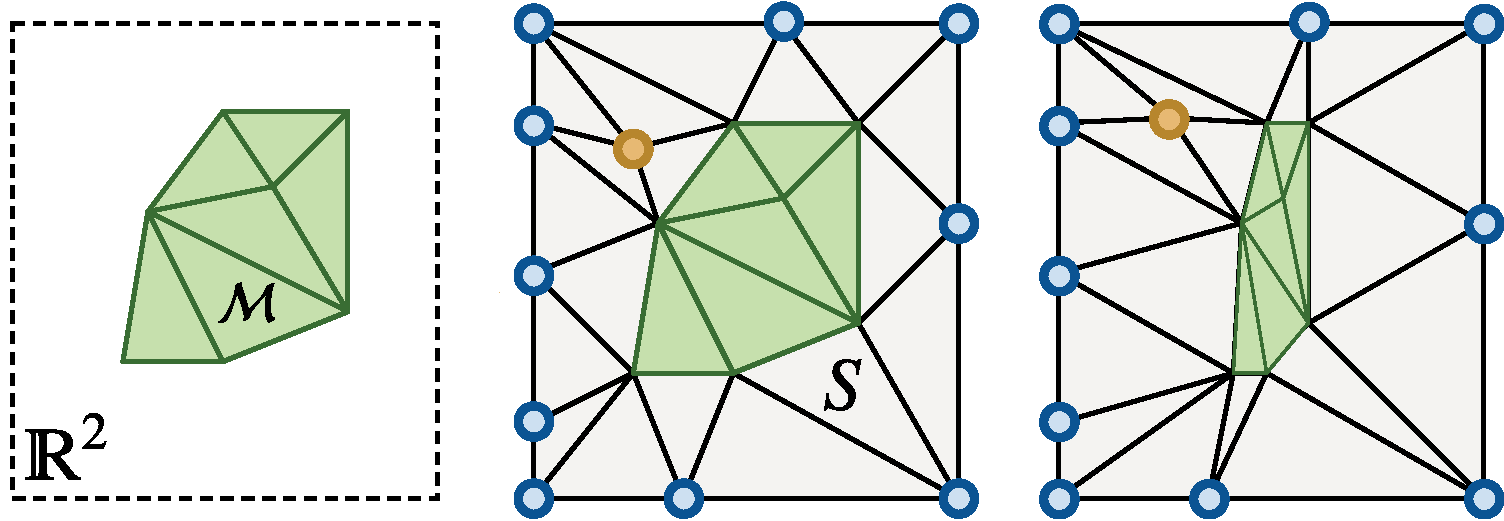
\includegraphics[width = \columnwidth]{scaf-tex/figs/scaffold_illustration}
\caption{The initial mesh $\Mesh$ (in green, left), is embedded in another mesh $D$ (in gray, middle) that covers a box in the ambient space and contains the same triangles as $\Mesh$. $D$ might contain additional points (orange). We denote the triangles that are in $D$ but not in $\Mesh$ as the scaffold $S$. Our algorithm deforms $D$, inducing a corresponding deformation on $\Mesh$ (right), while keeping the boundary (blue vertices) fixed and preventing changes in the triangle orientation.}
\label{scaf:fig:construction}
\end{figure}


 \paragraph{Variational Formulation} 
 Minimizing the distortion of $\Phi$ using the augmented map $\Psi$ poses an interesting challenge: what is the desired shape of the scaffold $S$? Ideally we would like the simplices in the scaffold to maintain their orientation and not affect the optimization in any other way. Such a requirement is difficult to model directly, since it is a discontinuous condition that is not well-suited for the variational framework that we would like to use to minimize $E_{\Mesh}$. 
 
 We propose a regularized version of this condition modeled with an energy $E_{\Mesh} (\Psi|_{S})$ that still diverges when elements change orientation and that mildly penalizes any non-rigid distortion.
 
 We choose a reweighted version of the symmetric Dirichlet energy $\Distort$~\cite{Smith:2015}, measured w.r.t. the Jacobian of the map $\Psi$ computed from the rest pose of $S$ for each simplex $f$,
\begin{equation}
    J_f := \nabla \Psi_f
\end{equation}
where $\Psi_f$ is the restriction of $\Psi$ over the simplex $f$, which is an affine map. We divide the energy of each scaffold simplex $f$ by its area $A_f$, and sum them up to obtain the final energy that favors an equal contribution regardless of the size of each scaffold simplex:
\begin{align}
    \begin{split}
    E_S(\Psi|_{S}) =&\sum_{f\in S} \frac{1}{A_f} \Distort(J_f) \\
    =&\sum_{f\in S} (\norm{J_f}_F^2 + \norm{J^{-1}_f}_F^2 -2d).
    \end{split}
\end{align}
The $-2d$ term ensures that the energy is 0 when $J_f = \mathbb{I}$. The map is then computed by summing the two terms:
\begin{align}
\begin{split}\label{eq:variational}
\min_{D} & \quad E_{\Mesh}(\Psi|_{\Mesh}) + \lambda E_{S} (\Psi|_{S}) \\
    \text{s.t.} & \quad \Psi|_{\partial D} \revision{\text{ is Identity}} \\ 
    & \quad \Psi \text{ preserves orientation}.
\end{split}
\end{align}
where $\lambda > 0$ is balancing the contribution of the two energies, decreasing as the optimization proceeds.

\paragraph{Iterative Regularization}
Solving this problem leads to a bijective and distortion minimizing map, but the regularizer will affect the stationary points of $E_{\Mesh}$, which is problematic, especially for large deformations.
%
To address this problem we iteratively minimize this energy, regenerating the scaffold at each iteration, and use the new scaffold as a rest pose for the regularization term $E_{S} (\Psi|_{S})$. This iterative procedure has two positive effects: (1) it acts as a proximal regularization term without inhibiting movement since the rest pose is updated at each iteration; (2) the meshing quality of the scaffold is high, which avoids locking configurations.

\paragraph{Interpolation Coefficient.}
We experimentally observed that our algorithm is robust to different choices of $\lambda$, generating indistinguishable results in most cases. However, $\lambda$ affects the convergence speed (Figure \ref{scaf:fig:different_weight}). We used $\lambda = \frac{1}{100}\frac{ E_{\Mesh}(\Psi|_{\Mesh})}{|S|}$ for all our experiments, where $|S|$ is the number of scaffold simplices.

\begin{figure}[h!]
\centering
    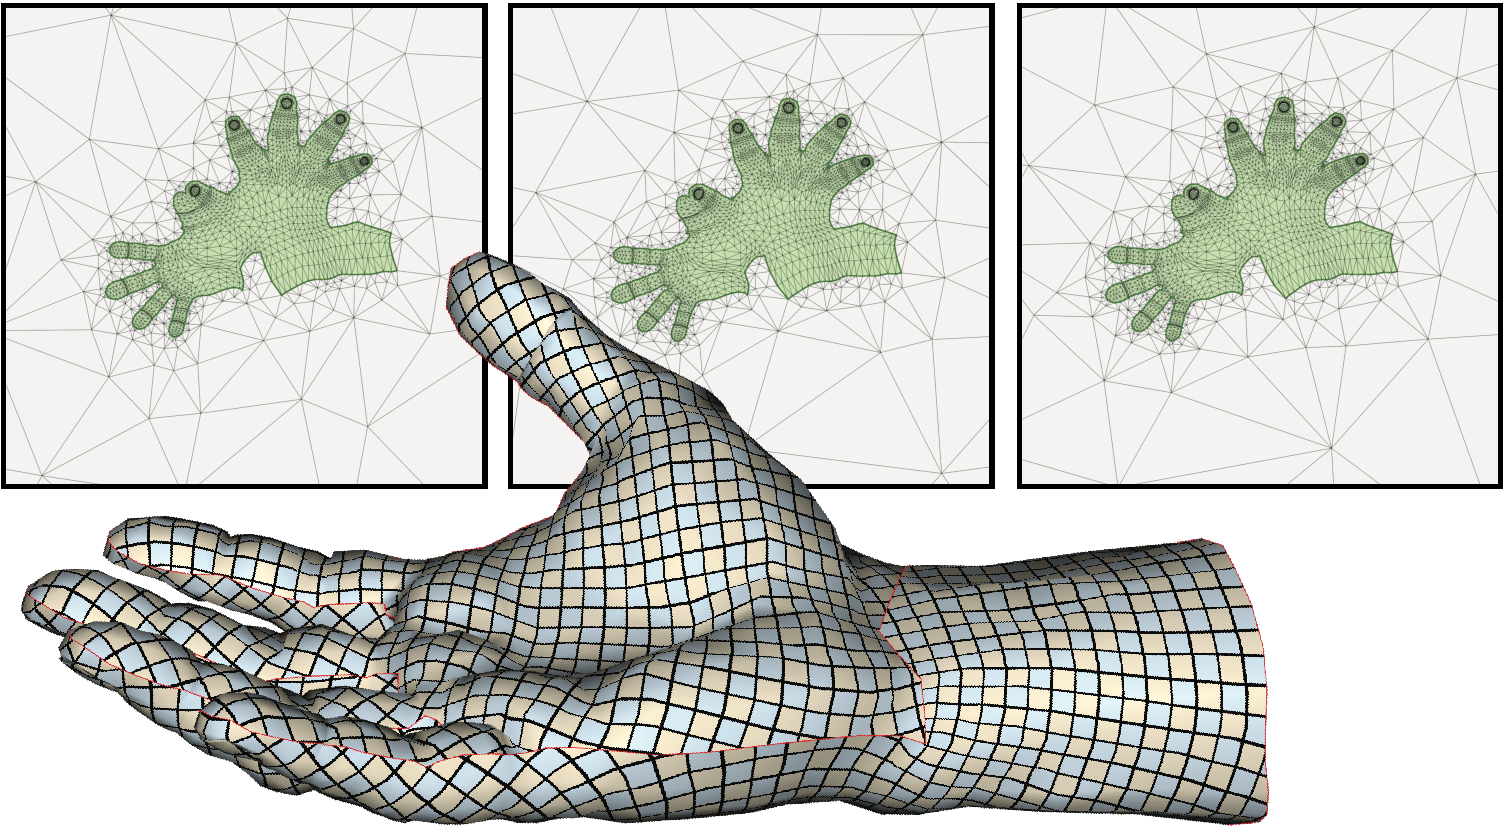
\includegraphics[width = \columnwidth]{scaf-tex/figs/hand_weight}
\caption{Different values of $\lambda$ do not affect the result, but they change the number of iterations needed. From left to right: we used a large weight (100x ours), our weight, and a small weight (0.01x ours). The optimization took 9,7, and 8 iterations, respectively, to reach the same energy level.}
\label{scaf:fig:different_weight}
\end{figure}

\paragraph{Solver.}
Since our energy is rotational invariant, we can minimize the energy with the same quadratic proxy proposed in SLIM \cite{Rabinovich:2017}, enriching the approach with the equality constraint needed to fix the boundary $\partial D$. We also employ the orientation-preserving line search \cite{Smith:2015} (with exact predicates \cite{Shewchuk:1996}) to ensure that no triangles can change orientation. Alternatively, other methods such as AQP \cite{Kovalsky:2016} could be used to minimize this energy. Since our approach changes the mesh connectivity at every iteration, AQP loses much of its advantages as the approximate \revision{H}essian must be recomputed at each iteration and not prefactored.  Therefore, our approach is an ideal fit for \cite{Rabinovich:2017}, which takes large steps at every iteration without relying on a constant, prefactored matrix at each iteration. For practical applications, SLIM iterations are sufficient to minimize the energy to acceptable levels. For two  stress tests (figures \ref{scaf:fig:recovering} and \ref{scaf:fig:smith}) we used the result of SLIM as a warm start for a Newton optimization (as suggested by \cite{Rabinovich:2017}), which quickly converges to a numerical minimum.

\subsection{Surface Parametrization}
Our framework can be used for many applications, one of which is computing a bijective surface parametrization from a 3D surface into the UV  plane. We follow \cite{Liu:2008} and assume that each 3D triangle $f^{3D}$ is equipped with a rigid transformation $R_f$ such that applying $R_f$ to $f^{3D}$ maps $f^{3D}$ to the plane. Given this transformed triangle $f$, we can now measure the distortion of the map using the Jacobian of the affine transformation (a $2\times2$ matrix) from $R_f(f^{3D})$ to $f$, the location of the triangle in the parametrization.

\paragraph{Initialization} Our method is initialized with Tutte's embedding algorithm~\cite{Tutte:1963}:
\[\Phi^0 : \Mesh^{3D} \rightarrow \Omega^0,\]
where $\Omega^0$ is a simplicial disk domain. Then we construct a larger rectangular domain $D^0 \supset \Omega^0$, where $\partial D^0$ is an axis-aligned rectangle, and use Triangle \cite{Shewchuk:1996} to triangulate the region in between.  We enforce a quality bound of $20^\circ$ to obtain a graded mesh that is coarse on the boundary and conforming the boundary of $\Omega^0$. This grading implicitly produces an approximate inverse distance  weighting of the scaffold space with respect to the error function, which enables a larger deformation per iteration. Then we define $\Psi: D^0 \rightarrow D \subset \mathbb{R}^{2}$ and restrict $\Psi |_{\partial D^0}$ to be the identity.
% \DP{Can we drop this?}We denote the vertex coordinates in $D^0$ by $U^0$, and augmented face set by $\matS$, i.e., $D^0 = (\matU^0, \matF\cup \matS)$.

\paragraph{Mesh Improvement}
At the end of each iteration, we improve the quality of the scaffold. The reason for maintaining a good mesh quality is two-fold. 
First, as observed in \cite{Zhang:2005, Muller:2015}, fixing the scaffold will potentially prevent movement. Secondly, the quality of the scaffold affects the condition of the linear system in SLIM \cite{Rabinovich:2017}: a higher  quality leads to larger and more efficient iterations.

We resort to Triangle \cite{Shewchuk:1996} to create the initial scaffold and to regenerate the scaffold mesh in the improvement step. Our experiments show that, in 2D, it is faster to generate the mesh from scratch at every iteration instead of trying to optimize the scaffold using local operations as suggested in \cite{Muller:2015}. Since our solver makes large steps in each iteration, the scaffold requires significant connectivity changes each iteration, which explains why regenerating the triangulation is faster than local operations. This is in stark contrast with physical simulation scenarios where each iteration represents a small time step and, thus, a minor change in the vertex positions.

We demonstrate the effectiveness of the remeshing strategy in Figure \ref{scaf:fig:recovering} where our method recovers from a large rotation --- note that the scaffold is updated during the iterations and always leaves space for the map to move freely.

\begin{figure}[h]
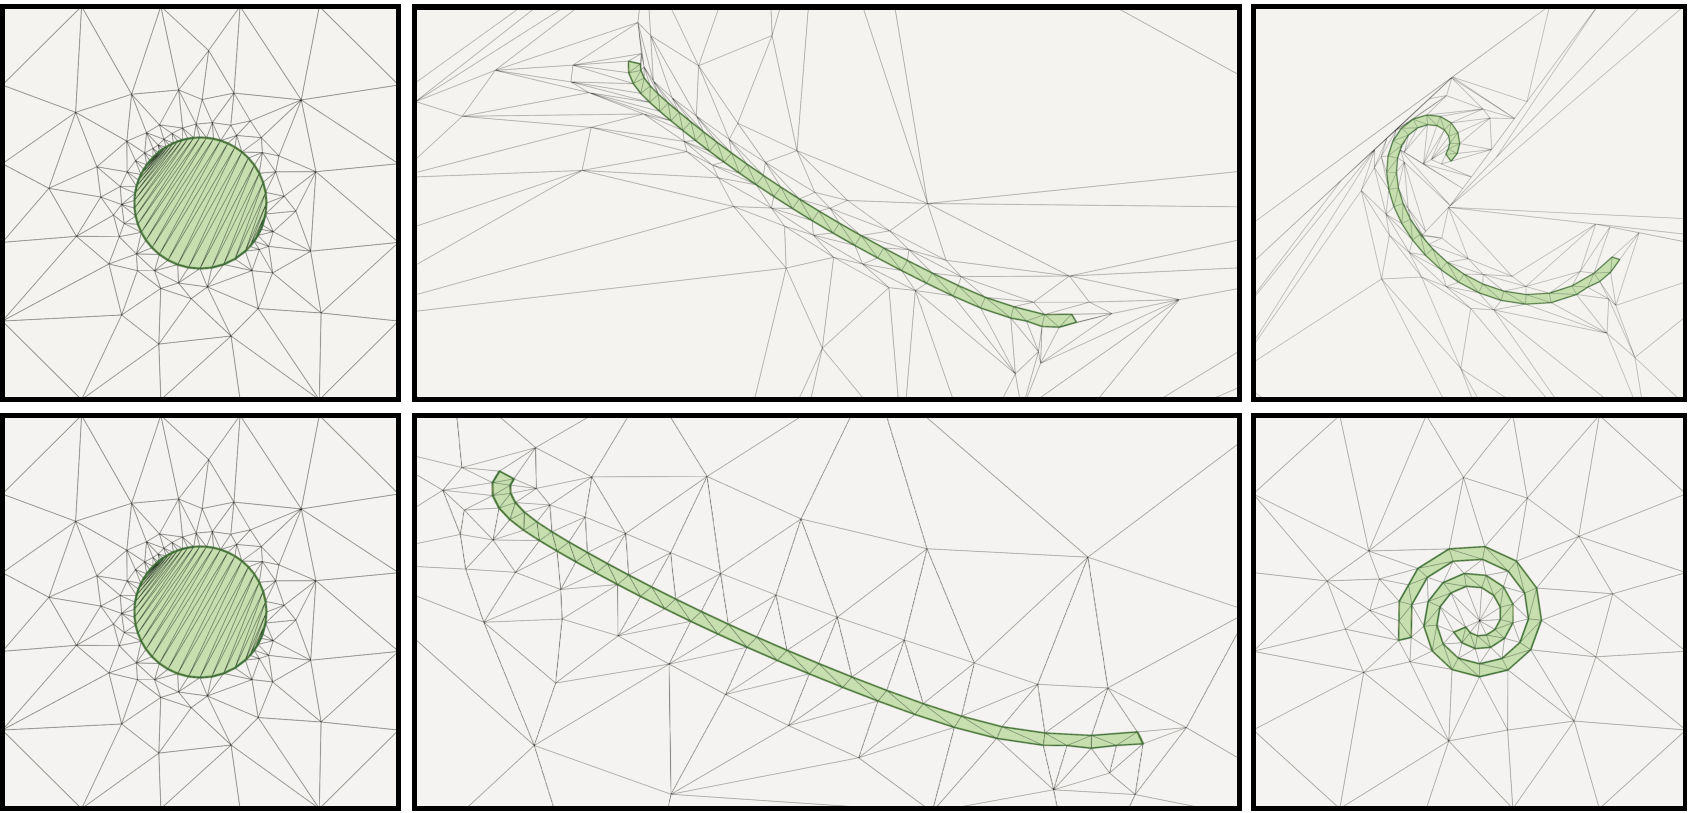
\includegraphics[width=\columnwidth]{scaf-tex/figs/coil-remeshing}
\caption{
\label{scaf:fig:recovering}
A bijective map from a circle (left) to a spiral (right) is computed without (top) and with (bottom) the iterative remeshing step. The slivers in the triangulation locks the optimization (top), preventing it from reaching the target shape.
% Recovering from a large rotation (up is remeshing: init, 30SLIM, 30 Newton; down is w/o reeshing 30 SLIM, 270 Newton) 
}
\end{figure}
\paragraph{Sliding \revision{\& Degeneracy Prevention}}
As the optimization proceeds and some of the boundary elements get closer, some of the scaffold triangles might (and often will) get smaller and smaller, restricting the amount of sliding that is allowed in one iteration as well as introducing numerical difficulties in computing the corresponding Jacobian $J_f$ \revision{whose singular values will approach infinity.}
% (Figure \ref{scaf:fig:slide}).  

To avoid this issue, we replace the degenerating target \revision{when computing its} Jacobian. For the triangles with an area smaller th\revision{an $\epsilon$, we use an equilateral triangle with area $\epsilon$ to compute the local Jacobian.} \revision{In our experiment,} we traverse through the boundary of the interior of the uv domain at the current iteration to find the minimum edge length $l$ \revision{and set} $\epsilon = \frac{l^2}{4}$.

A theoretical downside of this modification \revision{is that} it affects the distortion energy. We experimentally observed that the changes are negligible, and we thus used it for all our experiments. \revision{However, on the practical side}, it discourages fully degenerate elements --- this change, coupled with the orientation preserving line search \cite{Smith:2015}, makes our algorithm robust \revision{enough for the challenging stress tests shown in} Figure \ref{scaf:fig:miq_database}.
% \begin{figure}{h}
% 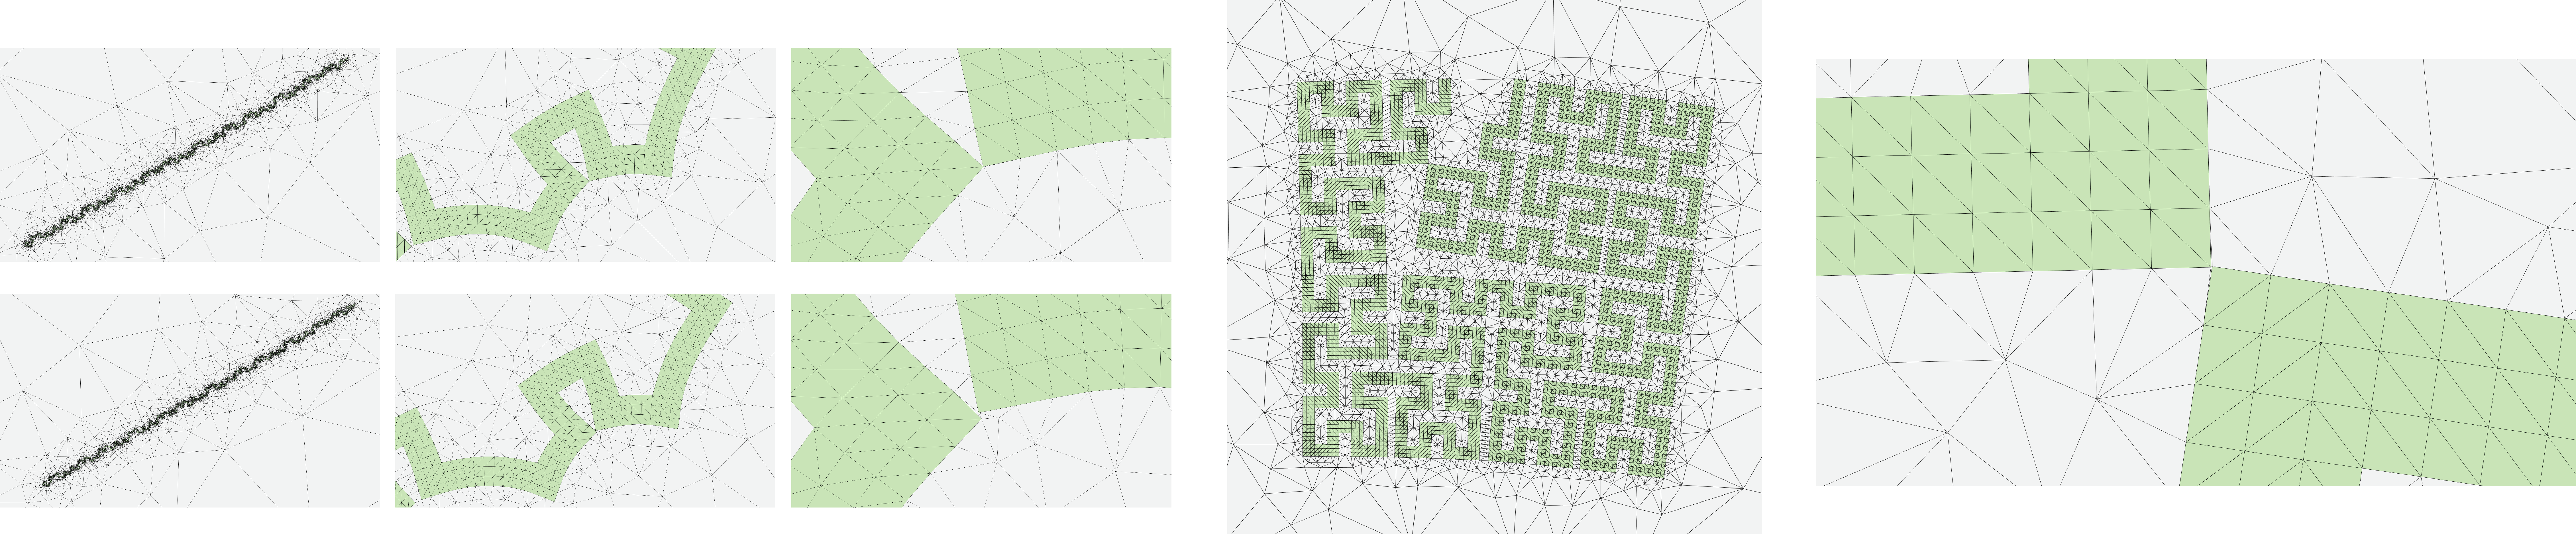
\includegraphics[width=8cm,height=4cm]{scaf-tex/figs/hilbert_area_threshold}
% \caption{
% Sliding example, one gets stuck the other one does not. \DP{TODO}}
% \label{scaf:fig:slide}
% \end{figure}

\subsection{Extension to 3D}

\revision{Our formulation naturally unifies bijective geometric optimization problems in 2D and 3D, so the} algorithm readily extends to the 3D case with only one major difference: the scaffold becomes a tetrahedral mesh, which is computationally more challenging to create and update.
\paragraph{\revision{Mesh Improvement}}
We use TetGen \cite{si2015tetgen} to generate the initial scaffold and the local operations proposed in \cite{Klingner:2009} to optimize the scaffold's quality in the subsequent iterations. 
%We describe our mesh improvement algorithm in details in Appendix \ref{appendix:improvement} \DP{TODO}.
%
It is unfortunately not possible to directly use TetGen at every iteration as we did with Triangle in the 2D case, since TetGen fails when boundaries get too close, which is common in our experiments.

\revision{
\paragraph{Guarantee} Similarly to the 2D case, we are guaranteed that no flipping or self-intersecting tetrahedra will occur since we are following an interior point strategy. Notice the contrast with Air Mesh \cite{Muller:2015} where only if penetration happens can the constraints be of effect. However, as pointed out in \cite{Dougherty2004}, the local operations we are performing may not be sufficient to explore the entire space of possible tetrahedralizations. %effective enough to explore the whole space of tessellation. 
Therefore, we cannot guarantee that the algorithm achieves the globally optimal solution.
}